\section{Introducción}
En el caso de las personas naturales, los impuestos pueden dividirse en impuestos directos e indirectos. Los primeros gravan el capital derivado de los ingresos o el patrimonio, mientras que los segundos gravan los actos de consumo. En particular, la teoría económica señala que los impuestos indirectos deberían ser bajos, pero en la práctica la mayor parte del recaudo proviene de ellos. Lo anterior es consecuencia de la facilidad en su recaudo, pues en el caso de los impuestos directos hay un incentivo perverso al subreporte, con el objetivo de minimizar el pago de impuestos. 

En este sentido, el presente trabajo busca, a partir del pronóstico de los ingresos, generar alertas tempranas e identificar individuos (contribuyentes) que estén reportando un ingreso menor al que, posiblemente, poseen --con el fin de disminuir el monto a pagar por concepto de impuestos--. % Señalar los resultados.

Así, la siguiente sección, \ref{Sec:datos} \nameref{Sec:datos}, detalla los datos que empleamos, haciendo énfasis en la construcción de las variables y la teoría económica o la racionalidad detrás de su inclusión. Posteriormente, las secciones \ref{Sec:perfilamiento} \nameref{Sec:perfilamiento} y \ref{Sec:brecha} \nameref{Sec:brecha} analizan posibles determinantes del nivel salarial. En particular, la primera de las anteriores señala la correlación de la edad sobre la senda salarial, mientras que la segunda subraya las diferencias salariales entre hombres y mujeres que no son consecuencia de habilidad o experiencia y que, por tanto, podrían considerarse como factores discriminatorios en el mercado laboral. Finalmente, la sección \ref{Sec:forecast} \nameref{Sec:forecast} realiza la estimación de los ingresos condicional en el análisis anterior más una serie de variables adicionales (y detalladas en la sección \ref{Sec:datos}).

\section{Datos} \label{Sec:datos}

% Acá va: a) descripción de los datos, incluir su propósito, fuente y muestra.\\ 
Los datos empleados en el presente documento provienen de la  Gran Encuesta Integrada de Hogares (GEIH) realizada en el año 2018 por el Departamento Administrativo Nacional de Estadística (DANE) en Colombia. Si bien esta encuesta es realizada en diferencias áreas metropolitanas, cabeceras municipales, y algunas zonas rurales del país, nosotros contamos con observaciones únicamente de la ciudad de Bogotá D.C., a partir de la extracción de datos realizada por el profesor \href{https://man-fern.github.io/}{Manuel Fernández} de la Universidad de los Andes. \\

%b) Descripción de procesamiento de adquisicón de datos: -web scraping -si hubo restricciones a la página a scrapear. \\
\subsection{\textit{Web scrapping}}
Realizamos \textit{web scrapping} sobre la \href{https://ignaciomsarmiento.github.io/GEIH2018_sample/}{página} del presente \textit{problem set}. La dificultad del ejercicio subyace en el hecho de que la página no contenía los datos, sino que contenía una referencia a otra página que sí contenía los datos. En ese sentido, fue necesario inspeccionar los elementos de la página para determinar la página y así sistematizar la extracción de las diez tablas. Para ver el código, remítase al \href{https://github.com/pisco-rolo/PS_1_ML}{repositorio en Github}. Sin embargo, a grandes rasgos, el paquete en el programa \texttt{R} utilizado para la extracción sistemática de los datos fue \texttt{rvest}, el cual no presentó restricción alguna para dicho proceso cuando fue ubicado el origen de las tablas dentro de la página \textit{web}.

\subsection{Descripción de las variables}
La base de datos posee 32,177 observaciones divididas en 10 pedazos de información --de tablas cuyo formato era \texttt{html}--.  Así, una vez los datos extraídos, procedemos a la limpieza de datos. Dado que el objetivo del presente documentos es realizar regresiones con el salario laboral, decidimos mantener solo las observaciones de individuos que sean mayores de edad (es decir, edad mayor o igual a 18 años). Así mismo, nos quedamos solo con las personas que percibieron ingresos laborales. Esto redujo la muestra a un total de 9,892 observaciones. Posteriormente, formateamos a las variables. En otros términos, agregamos etiquetas a las variables y las declaramos como factores en \texttt{R}, de forma tal que podamos emplear una codificación \textit{one-hot-encoding} para la correcta implementación de la regresión\footnote{Por ejemplo, no tiene sentido dejar una variable discreta de estrato socieconómico que camina sobre los valores del uno al seis e incluirla como variable explicativa, en tanto ello asumiría un crecimiento salarial lineal a través de los estratos. En su lugar, el \textit{one-hot-encoding} crea seis variables binarias, donde cada una de ellas toma el valor de uno (1) si el $i$--ésimo trabajador o trabajadora vive en el estrato $j$.}. 

A continuación, en el Cuadro \ref{Tab:variables}, describimos las variables que consideramos relevantes para el presente ejercicio.

\begin{longtable}{|>{\raggedright\arraybackslash}p{.35\linewidth}|p{.65\linewidth}|}
    % ------------------------------------------------------------------------------------
    % Personalización de la tabla.
    % ------------------------------------------------------------------------------------
    % Encabezado de la primer vez que aparece la tabla.
    \caption{Variables empleadas en el análisis.}
    \label{Tab:variables}
    \hline 
    \textbf{Variable} & \textbf{Descripción} \\
    \hline
    \endfirsthead
    % Encabezado de las próximas veces que aparece la tabla en otra página.
    \multicolumn{2}{c}%
    {{\bfseries \tablename\ \thetable{}. } (Continuación).} \\
    \hline
    
    \textbf{Variable} & \textbf{Descripción} \\
    \hline
    \endhead
    
    % Pie de página de una tabla al terminar y continuar en la próxima tabla.
    \multicolumn{2}{r}{{Continúa en la siguiente página.}} \\ 
    \endfoot
    
    % Pie de página cuando es el final de la tabla y no continúa en la siguiente.
    \hline
    \endlastfoot
    % ------------------------------------------------------------------------------------
    % Contenido de la tabla.
    % ------------------------------------------------------------------------------------
    \textbf{Variable de interés}. Salario laboral (nominal) mensual del $i$--ésimo individuo dividido por el número total de horas trabajadas en el mes. Incluye propinas y comisiones. 
    $y_{i} = \ln \left( \frac{\text{Salario mensual}}{\text{Número de horas de trabajo}} \right)$

    & Variable numérica a nivel individuo. Esta variable la tomamos ya construida por el profesor \href{https://man-fern.github.io/}{Manuel Fernández} y brindada en la base de datos. Dada la log-normalidad del salario por hora, tomamos una transformación logarítmica. \\
    \hline
    \textbf{Variable explicativa.} Estrato socioeconómico.  
    & Variable categórica que convertimos en 6 dummys. El orden de los estratos importa para la clasificación, donde 1 es el estrato más bajo y 6, el más alto, o de mayor poder adquisitivo.
    Información según el estrato definido en el recibo de energía eléctrica.  Esperaríamos una correlación positiva entre estrato más alto e ingreso.  \\
    \hline
    \textbf{Sexo} 
    & Variable categórica donde la dummy igual a 1 indica el sexo femenino y 0, el sexo masculino.   \\
    \hline
    \textbf{Posición dentro del hogar} 
    & Variable categórica que convertimos en 4 dummys. Puede ser Jefe de hogar, pareja del jefe, descendiente de este, u otro. Podríamos suponer que ser Jefe de hogar implica mayor responsabilidad, y por lo tanto, debería tener mayor ingreso laboral en una familia promedio. \\
    \hline
    \textbf{ Nivel educativo más alto}
    & Variable categórica que convertimos en 6 dummys. Puede ser ningún nivel educativo, preescolar, primaria, secundaria, bachillerato o superior. Esperaríamos que a mayor nivel educativo, haya mayor ingreso laboral.  \\
    \hline    
    \textbf{Ocupación} 
    & Variable categórica, dada la muestra se convirtió en 4 dummys. Puede ser empleado doméstico, jornalero, obrero/empleado del gobierno u obrero/empleado del sector privado. En este caso, el efecto esperado es diverso, dependiendo de la ocupación. \\
    \hline
    \textbf{Empleo formal o informal}  
    & Variable categórica, donde 1 indica que el empleo es formal y 0, lo contrario. Esperaríamos mayor ingreso en promedio en el sector formal dada la estructura de la economía colombiana.   \\
    \hline
    \textbf{Tamaño de la empresa} 
    & Variable categórica que convertimos en una dummy donde 1 indica si trabaja en una microempresa, y 0 si trabaja en una empresa pequeña, mediana o grande. En este caso, esperaríamos que haya una relación negativa si trabaja en una microempresa promedio.   \\
    \hline
    \textbf{Edad} 
    & Variable numérica. Incluye solo individuos mayores de edad, es decir desde los 18 años en adelante.    \\
    \hline
\end{longtable}
    
\vspace{-0.5cm}
\begin{center}
    \textbf{Fuente}. Elaboración propia, con base en base en los datos de la GEIH 2018.
\end{center}

\subsection{Estadística descriptiva}
En el Cuadro \ref{tab:descriptiva}, mostramos la estadística descriptiva de los datos obtenidos.

%%%%%%%%%%%%%%%%%%%%%%%%%%%%%%%%%%%%%%%%%%%%%%%%%%%%%%%
%%%%%%%%%%%%%%%%%%%%%%%%%%%%%%%%%%%%%%%%%%%%%%%%%%%%%%%
%%%%%%%%%%%%%%%%%%%%%%%%%%%%%%%%%%%%%%%%%%%%%%%%%%%%%%%
\begin{table}[H]
\caption{Estadísticos descriptivos}
\label{tab:descriptiva}
\centering
\footnotesize
\begin{longtable}{lc}
\toprule
\textbf{Variable} & \textbf{N = 9,892} \\ 
\midrule
\textbf{Estrato socioeconómico,}  &  \\ 
    Uno & 1,039  (11\%) \\ 
    Dos & 4,380  (44\%) \\ 
    Tres & 3,483  (35\%) \\ 
    Cuatro & 602  (6.1\%) \\ 
    Cinco & 167  (1.7\%) \\ 
    Seis & 221  (2.2\%) \\ 
\textbf{Sexo,}  &  \\ 
    Hombre & 4,973  (50\%) \\ 
    Mujer & 4,919  (50\%) \\ 
\textbf{Posición dentro del hogar,}  &  \\ 
    Jefa o jefe del hogar & 4,418  (45\%) \\ 
    Pareja de la cabeza del hogar & 2,000  (20\%) \\ 
    Descendiente de la cabeza del hogar & 2,322  (23\%) \\ 
    Otro & 1,152  (12\%) \\ 
\textbf{Nivel educativo más alto alcanzado,}  &  \\ 
    Ninguno & 46  (0.5\%) \\ 
    Primaria & 1,009  (10\%) \\ 
    Secundaria & 940  (9.5\%) \\ 
    Bachillerato & 3,419  (35\%) \\ 
    Superior & 4,478  (45\%) \\ 
\textbf{Ocupación,}  &  \\ 
    Empleado doméstico & 563  (5.7\%) \\ 
    Jornalero & 1  (<0.1\%) \\ 
    Obrero del gobierno & 571  (5.8\%) \\ 
    Obrero del sector privado & 8,757  (89\%) \\ 
\textbf{Empleo formal o informal,}  &  \\ 
    Formal & 7,592  (77\%) \\ 
    Informal & 2,300  (23\%) \\ 
\textbf{Tamaño de la empresa,}  &  \\ 
    Empresa pequeña, mediana, o grande & 7,646  (77\%) \\ 
    Microempresa & 2,246  (23\%) \\ 
\textbf{Edad} &  \\ 
    Promedio (Desviación std) & 36 (12) \\ 
    Mínimo y máximo & (18, 86) \\ 
\textbf{Salario por hora}                                                                                                                                                                                                                                                                                                                                                                                                                                                                                                                                                                                                                                                                                                                                                                                                                                                                                                                             &  \\ 
    Promedio (Desviación std) & 8,822 (12,886) \\ 
    Mínimo y máximo & (327, 350,583) \\ 
\bottomrule
\end{longtable}



\begin{center}
    \textbf{Fuente}. Elaboración propia, con base en base en los datos de la GEIH 2018. \\
    \scriptsize{\textit{Nota.} La base de datos tiene un total de 9,892 observaciones. Si la variable es categórica, presentamos el número de observaciones en dicha categoría, así como el porcentaje de observaciones en dicha categoría con respecto al total de observaciones entre paréntesis. Si la variable es numérica (edad y salario por hora), presentamos el valor promedio, la desviación estándar, y los valores mínimos y máximos.}
\end{center}

\end{table}

%%%%%%%%%%%%%%%%%%%%%%%%%%%%%%%%%%%%%%%%%%%%%%%%%%%%%%%
%%%%%%%%%%%%%%%%%%%%%%%%%%%%%%%%%%%%%%%%%%%%%%%%%%%%%%%
%%%%%%%%%%%%%%%%%%%%%%%%%%%%%%%%%%%%%%%%%%%%%%%%%%%%%%%

% comentar de todas las variables, sus respectivo porcentaje. y la media y desviación de las numéricas. 
Respecto a los datos en la tabla anterior, todas las variables cuentan con las observaciones completas (no hay missing values). En específico, respecto a los estratos socioeconómico, vemos que el grueso de la muestra se concentra entre los estratos dos y tres con 44\% y 35\%, respectivamente. Adicionalmente, le siguen el estrato uno (11\%), el cuatro (6.1\%), el cinco (1.7\%) y el seis (2.2\%). \\

Además, la variable sexo está igualmente distribuida en el porcentaje (50\% hombres y 50\% mujeres), con una ligera variación de 54 hombres más que mujeres. Asimismo, contamos con la variable posición dentro del hogar\footnote{En la encuesta, esta variable viene de la pregunta: ¿cuál es el parentesco de ...Con el jefe o jefa del hogar?.} donde el 45\% de individuos es jefa o jefe de hogar. Por otro lado, las parejas de estos representan el 20\%, los descendientes (hijos) de la cabeza de hogar son el 23\%, y otros (pensionistas, nietos, otros parientes, trabajadores o empleados domésticos) son solo el 12\%. \\ 

En cuanto al nivel educativo más alto alcanzado, la mayoría de la muestra posee o educación superior(45\%) o bachillerato(35\%), mientras el resto se divide entre los que solo cuenta con secundaria(9.5\%), primaria (10\%) o ninguna educación (0.5\%). Por otra parte, la distribución de las ocupación está claramente marcada por obreros/empleados del sector privado quienes representan un 89\%. Le siguen los obreros/empleados del gobierno (5.8\%) con una proporción muy parecida a la de los empleados domésticos (5.7\%). Por últimos, solo hay un jornalero que representa menos de 0.1\% de la muestra. Por último, los trabajadores del sector formal representan el 77\% y del sector informal solo el 23\%. Aunque esto pueda parecer raro, por el conocimiento general de la economía colombiana y su alta informalidad, sin embargo, dado que la muestra es solo de Bogotá D.C., entonces si es posible encontrar dicha cifra coherente.  \\

En cuanto a las variables numéricas, la edad promedio de los participantes es de 36 años con una desviación estándar de 12, un mínimo de 18 años y un máximo de 86 años. Esto indica una población relativamente joven en la parte productiva de la ciudad. Adicionalmente, los salarios por hora por actividad princiapl en promedio son de 8,882 pesos con una desviación de 12,886, un mínimo de 327 y un máximo de 350,583 pesos. 



\section{Perfilamiento salarial} \label{Sec:perfilamiento}
En esta sección se busca encontrar el perfilamiento del salario y edad "\textit{Wage-Age}; con el fin de estimar el siguiente modelo:
\begin{equation}
    log(w) = \beta_1 + \beta_2 Age +\beta_3 Age^2 + u
\end{equation}
Donde Age es mayor o igual a 18 años.\\ 

a) Resultado de tabla de Regresión \\
[5cm]

\begin{table}[H]
\label{tab:Cuadro 3}
\centering
\footnotesize

% Table created by stargazer v.5.2.3 by Marek Hlavac, Social Policy Institute. E-mail: marek.hlavac at gmail.com
% Date and time: lun., sept. 18, 2023 - 5:20:29 p. m.
% Requires LaTeX packages: dcolumn 
\begin{table}[!htbp] \centering 
  \caption{} 
  \label{} 
\begin{tabular}{@{\extracolsep{5pt}}lD{.}{.}{-3} } 
\\[-1.8ex]\hline 
\hline \\[-1.8ex] 
 & \multicolumn{1}{c}{\textit{Dependent variable:}} \\ 
\cline{2-2} 
\\[-1.8ex] & \multicolumn{1}{c}{log(num\_salarioHora)} \\ 
\hline \\[-1.8ex] 
 num\_edad & 0.067^{***} \\ 
  & (0.004) \\ 
  & \\ 
 I(num\_edad$\hat{\mkern6mu}$2) & -0.001^{***} \\ 
  & (0.00004) \\ 
  & \\ 
 Constant & 7.374^{***} \\ 
  & (0.068) \\ 
  & \\ 
\hline \\[-1.8ex] 
Observations & \multicolumn{1}{c}{9,892} \\ 
R$^{2}$ & \multicolumn{1}{c}{0.044} \\ 
\hline 
\hline \\[-1.8ex] 
\textit{Note:}  & \multicolumn{1}{r}{$^{*}$p$<$0.1; $^{**}$p$<$0.05; $^{***}$p$<$0.01} \\ 
\end{tabular} 
\end{table} 


\begin{center}
    \textbf{Fuente}. Elaboración propia, con base en base en los datos de la GEIH 2018. \\

\end{center}

\end{table}

b) Interpretación de los coeficiente.\\ 

Definimos Age como la variable de Edad de las personas \textit{num-edad}. \\

\begin{itemize}
    \item Para Edad, el coeficiente es 0.067 (p<0.01); lo que en principio indicaría que en promedio, un incremento de una unidad en la edad de un trabajador se asocia con un aumento del 6.7 \% en el salarios por hora. Este resultado es altamente significativo. Sin embargo, dado que no es una regresión lineal simple, no es tan intuitiva su interpretación ya que debemos tener en cuenta $\beta_3$, que es el coeficiente del cuadrado de la Edad. \\
    
    \item Para $Edad^2$, el coeficiente es -0.001 (p<0.01), lo que nos muestra este coeficiente es que dada la forma cuadrática de la función, la forma es cóncava. \\
    
\end{itemize}

Por otro lado, el coeficiente de determinación (R²) del modelo es 0.044, lo que significa que el modelo explica aproximadamente el 4.4\% de la variabilidad en el logaritmo de los salarios por hora. Aunque es un valor bajo, sugiere que la edad y la edad al cuadrado contribuyen significativamente a la explicación de las diferencias en los ingresos por hora. \\
 [5 cm]

El análisis revela que la edad de los trabajadores tiene un impacto significativo en sus ingresos por hora. Es importante destacar que, aunque el modelo es significativo, todavía queda una gran cantidad de variabilidad en los ingresos por hora que no se ha explicado, lo que sugiere que otros factores también desempeñan un papel importante.\\

c) Estimación del Pico de Edad y Errores de Confianza.\\

Para estimar el ``pico de edad'' en relación con el perfil de ingresos por edad y calcular sus errores de confianza, implementamos la técnica de Bootstrap. El "pico de edad" se define como la edad en la que los ingresos alcanzan su punto máximo según nuestro modelo de regresión. Inicialmente ajustamos un modelo de regresión de ingresos logarítmicos en función de la edad, incluyendo una componente cuadrática para capturar posibles no linealidades en la relación.

La fórmula para el ``pico de edad'' se deriva del modelo como: $-\frac{B_1}{2 \cdot B_2}$, donde $B_1$ y $B_2$ son los coeficientes estimados de la regresión. Sin embargo, dado que trabajamos con muestras de datos limitadas, nuestras estimaciones podrían estar sujetas a variaciones debido a la aleatoriedad inherente a los datos.

Para abordar esta variabilidad, implementamos la técnica de bootstrap, que implica realizar múltiples remuestreos de nuestros datos originales. En cada iteración de Bootstrap, ajustamos nuevamente el modelo de regresión y calculamos los coeficientes $B_1$ y $B_2$. Luego, utilizamos estos coeficientes para estimar el ``pico de edad'' en esa muestra bootstrap específica.

Repetimos este proceso numerosas veces (en este caso, 2000 iteraciones) para obtener una distribución de ``pico de edad'', a partir de la cual podemos calcular intervalos de confianza. Los valores resultantes del Bootstrap nos proporcionaron una estimación puntual del ``pico de edad'' y, al calcular los percentiles 2.5\% y 97.5\% de la distribución, pudimos establecer intervalos de confianza al 95\% para el ``pico de edad''. Así, dada esta muestra de los bogotanos, el peack age es a la edad de 45.31 años y los intervalos de confianza están entre los 44.099 años y los 46.833 años de edad.


\begin{figure}[ht]
  \centering
  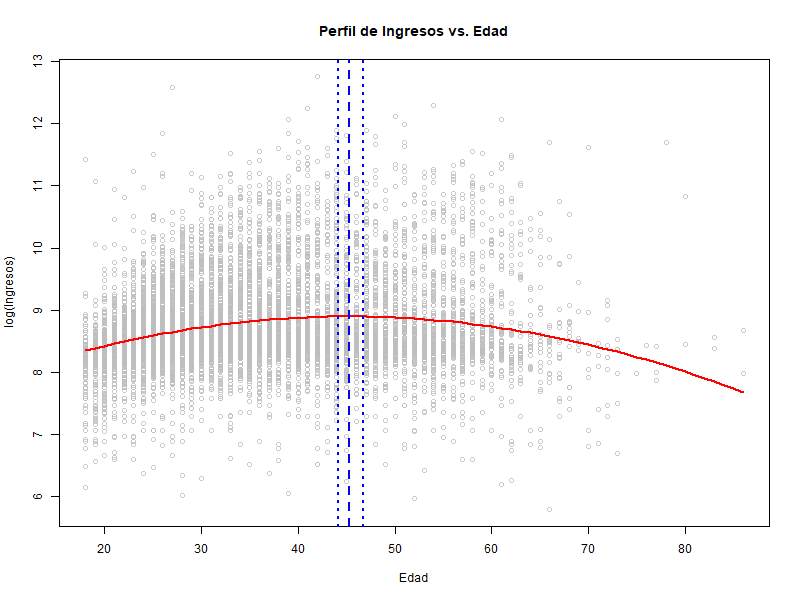
\includegraphics[width=1.1\textwidth]{Imagenes/perfil_ingresos_vs_edad.png}
  \caption{Perfil de Ingresos vs. Edad}
  \label{fig:perfil_ingresos}
\end{figure}

En la Figura \ref{fig:perfil_ingresos} se muestra el perfil de ingresos por edad, con el ``pico de edad'', estimado y sus intervalos de confianza resaltados.\\

Por lo tanto, con esta técnica, no solo pudimos estimar el ``pico de edad'' sino también cuantificar la incertidumbre asociada a esta estimación. De esta manera, podemos entender que es razonable dicho intervalo, ya que una persona en promedio tendría aproximadamente 20 años de experiencia, lo cual le debería alcanzar para obtener mayores ingresos. Adicionalmente, su capacidad física no debería limitarle el esfuerzo de trabajar, lo cual cambiaría en los siguientes años (de los 50 en adelante), y por ello también su declive. Esto nos permite tener una comprensión más completa de la relación entre la edad y los ingresos y brinda información valiosa para la toma de decisiones en la recolección de impuestos por ejemplo.



\section{Brecha de ingresos por género} \label{Sec:brecha}
a) Con el fin de encontrar cómo cambia el salario dado que se es hombre o mujer, estimamos inicialmente la siguiente regresión:
\begin{equation}
    log(w) = \beta_1 + \beta_2 Female + u
\end{equation}
Donde Female es 1 si el individuo es mujer. Los resultados de la regresión se muestran en el cuadro 5:
Esta regresión nos indica que el hecho de ser mujer disminuye el salario en 4.46\% con respecto a ser hombre con una significancia del 1\%. \\
[1cm]
b) Esta primera estimación se podría mejorar añadiendo los controles que fueron planteados inicialmente y que se especifican en el cuadro 5 con el fin de hacer mejores predicciones dadas las correlaciones que hay entre el salario y estas variables adicionales. Para ello estimaremos el valor del gap salarial y su error estándar mediante FWL y luego con FWL pero calculando su error estándar con boostrap.
\begin{itemize}
    \item FWL: Después de calcular las dos etapas, los resultados de la regresión se muestran en la segunda fila del cuadro 5:    
    Este resultado difiere en su error estándar del resultado de haber calculado el gap con una simple regresión lineal con los mismos controles debido a que tiene más grados de libertad y por tanto tenemos un error estándar ligeramente más pequeño. Esto nos muestra que ser mujer disminuye el salario en un 8.7\% con respecto a los hombres una vez tenemos en cuenta los controles mencionados en el cuadro 5.
    \item FWL con boostrap: En este caso mediante boostrap obtenemos que el valor del gap es de -0.087 y el error estándar es de 0.011. Mientras que el valor del gap es el mismo, la diferencia entre los errores estándar se da porque cuando FWL corre la regresión de las dos etapas, asume homocedasticidad , lo que no es cierto. Si en FWL corrigieramos esa heterocedasticidad, obtendríamos el mismo resultado en los errores estándar tanto por FWL como por boostrap.
\end{itemize}

\begin{table}[H]
\centering

% Table created by stargazer v.5.2.3 by Marek Hlavac, Social Policy Institute. E-mail: marek.hlavac at gmail.com
% Date and time: lun., sept. 18, 2023 - 2:43:00 p. m.
% Requires LaTeX packages: dcolumn 
\begin{table}[!htbp] \centering 
  \caption{} 
  \label{} 
\begin{tabular}{@{\extracolsep{5pt}}lD{.}{.}{-3} D{.}{.}{-3} } 
\\[-1.8ex]\hline 
\hline \\[-1.8ex] 
 & \multicolumn{2}{c}{\textit{Variable dependiente:}} \\ 
\cline{2-3} 
\\[-1.8ex] & \multicolumn{1}{c}{log(Salario Residuo)} & \multicolumn{1}{c}{log(Salario por hora)} \\ 
\\[-1.8ex] & \multicolumn{1}{c}{(1)} & \multicolumn{1}{c}{(2)}\\ 
\hline \\[-1.8ex] 
 Sexo Residuo & -0.087^{***} &  \\ 
  & (0.011) &  \\ 
  & & \\ 
 Dummy = 1 si es Mujer &  & -0.045^{***} \\ 
  &  & (0.015) \\ 
  & & \\ 
 Constante & -0.000 & 8.747^{***} \\ 
  & (0.005) & (0.010) \\ 
  & & \\ 
\hline \\[-1.8ex] 
Observaciones & \multicolumn{1}{c}{9,892} & \multicolumn{1}{c}{9,892} \\ 
R$^{2}$ & \multicolumn{1}{c}{0.006} & \multicolumn{1}{c}{0.001} \\ 
\hline 
\hline \\[-1.8ex] 
\end{tabular} 
\end{table} 

\scriptsize{\begin{flushleft}\textit{Nota:} Incluye controles de estrato socioeconómico, posición dentro del hogar, nivel educativo más alto alcanzado, ocupación, empleo formal, tamaño de la empresa y edad *** $p<0.01$, ** $p<0.05$, * $p<0.1$.  \end{flushleft}} 
\end{table}

Vemos que el $R^2$ de las ecuaciones difieren significativamente cuando se incluyen los controles en el cuadro 5. A medida que aumentan los controles, el $R^2$ va aumentando, lo que es coherente con el resultado del cuadro.

Para encontrar la diferencia entre en los picos para cada sexo, hacemos dos regresiones, una con los datos para los hombres y otra para las mujeres, luego hacemos las predicciones correspondientes y al igual que en el punto anterior, para cada regresión encontramos mediante boostrap $-\frac{B_1}{2 \cdot B_2}$ con sus intervalos de confianza hallando así los picos. Aunque los resultados para ambas regresiones son estadísticamente significativas, es decir, la edad explica parte de la varianza del logaritmo del salario, hay una gran parte de la varianza que no es explicada.

\begin{figure}[H]
\caption{Brecha de ingresos por sexo}
\label{gen_gap}
\centering
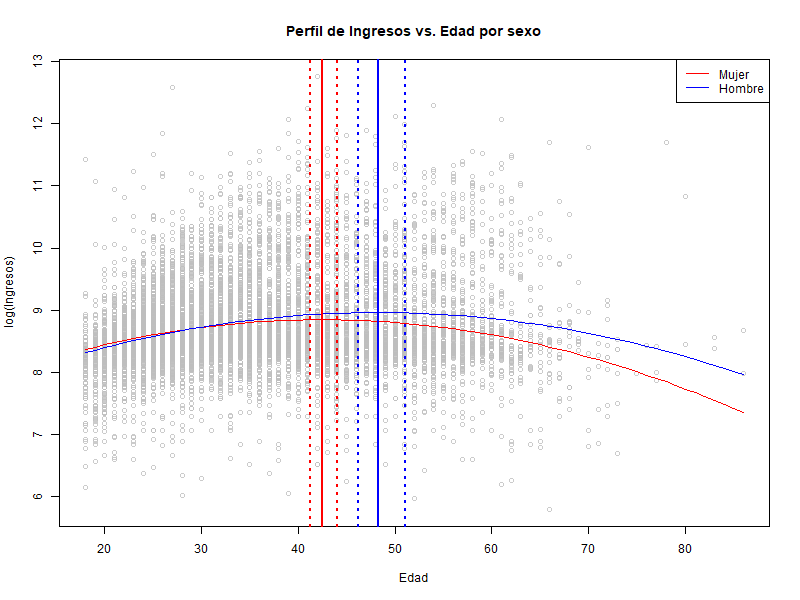
\includegraphics[scale=0.6]{Imagenes/earnings_gen_gap.png}
\scriptsize{\begin{flushleft}\textit{Nota:} Lineas verticales continuas: Peak ages para cada sexo. Lineas verticales punteadas: Intervalos de confianza.  \end{flushleft} }
\end{figure}

En la gráfica podemos notar que el valor peak para los hombres es de 48.272 y para las mujeres el valor peack es de 42.508. La gráfica nos muestra además que los intervalos de confianza entre ambos sexos no se tocan entre ellos, por lo que hay una una diferencia significativa entre ambas edades.

Por otro lado, ya que esta gráfica solo ha tenido en cuenta la edad y el $R^2$ es tan bajo, seguramente la inclusión de más predictores podría mejorar mucho la predicción. Es posible que cuando se hayan hecho las encuestas hayan hombres que no estén por estar en el trabajo por ejemplo y por tanto se cree selección. 

\section{Predicción de ingresos}  \label{Sec:forecast}
En los casos anteriores nos enfocamos en un análisis inferencial. En particular, \textit{i.}) si existe discriminación en el mercado laboral por género, y \textit{ii.}) si el salario responde al tiempo en el mercado laboral y si este alcanza un pico para alguna edad en particular. En la presente sección el objetivo pasa a ser predicción.

Para ello, tomamos un enfoque de validación, con una proporción del 70\% de los datos para el entrenamiento y el 30\% restante para la evaluación\footnote{Por la naturaleza aleatoria de este procedimiento, computacionalmente aprovechamos la ventaja de los números pseudo-aleatorios para que los resultados sean replicables posteriormente. Así, definimos una semilla numérica en el archivo principal, tal que los resultados posteriores se mantengan.}. Así, una vez partida la base de datos, estimamos siete modelos. En particular, los dos modelos estimados previamente, más cinco modelos adicionales. A continuación se detalla la precisión en la predicción de los modelos bajo la raíz del error cuadrático medio.

% latex table generated in R 4.3.1 by xtable 1.8-4 package
% Mon Sep 18 12:48:13 2023
\begin{table}[H!]
\centering
\caption{Resultados de la raíz del error cuadrático medio para los siete modelos.} 
\label{Tab:RMSE}
\begin{tabular}{cccc}
  \hline
Modelo & RMSE (ln) & RMSE (exp del ln) & RMSE (nivel) \\ 
  \hline
Edad & 0.716 & 2.05 & 12604 \\ 
  Género & 0.730 & 2.08 & 12739 \\ 
  Educación & 0.635 & 1.89 & 11929 \\ 
  Familiar & 0.610 & 1.84 & 10631 \\ 
  Empresarial & 0.638 & 1.89 & 12190 \\ 
  Todo & 0.494 & 1.64 & 9661 \\ 
  Interacción & 0.493 & 1.64 & 9655 \\ 
   \hline
\end{tabular}
\end{table}

\begin{center}
    \textbf{Fuente}. Elaboración propia, con base en base en los datos de la GEIH 2018. \\
    \scriptsize{\textit{Nota.} La variable dependiente está medida en el logaritmo natural, por lo que la interpretación del RMSE es complicada (columna 2). En particular, incluimos el exponencial del valor calculado (columna 3), y el RMSE de la variable en nivel (columna 3). Para este último cambio tomamos el exponencial de los valores $\ln (y)$ y $\hat{\ln (y)}$, teniendo en cuenta que una transformación log-normal no revierte al valor esperado con solamente el exponencial (es decir, al tomar el exponencial de la variable estimamos la mediana), sino que le sumamos a $y$ la varianza dividida por dos para que sea un estimador insesgado de la media.}
\end{center}

En el Cuadro \ref{Tab:RMSE}, las dos primeras filas corresponden a los modelos implementados en los puntos anteriores. La tercera fila hace referencia a un modelo que emplea, únicamente, variables relacionadas con la educación del $i$--ésimo individuo (en particular, el nivel de educación más alto alcanzado). La cuarta fila denota un modelo que utiliza variables relacionadas con características del hogar o la familia, como lo son el estrato donde vive y la posición al interior (por ejemplo, si es cabeza del hogar, la pareja, o un descendiente). La quinta fila hace referencia a las características de la empresa, como si es un trabajo formal, la empresa es microempresa, y en qué sector se desempeña la empresa. Finalmente, las últimas dos filas hacen referencia a modelos donde se incluyeron todas las variables anteriormente mencionadas, y en particular el último modelo incluye efectos heterogéneos (modelados a través de interacciones entre los regresores) entre el género de la persona y su ocupación, y entre el género de la persona y su nivel educativo.  

Una vez explicados los modelos implementados, merece la pena señalar que la segunda columna del Cuadro \ref{Tab:RMSE} es la raíz cuadrada del ratio al cuadrado promedio entre los valores observados y los estimados, pues:
\begin{align}
    RMSE & = \sqrt{\frac{\sum_{i=1}^{N} (\ln (y_{i}) - \hat{\ln (y)}_{i})^{2}}{N}} \nonumber \\
    & = \sqrt{\frac{\sum_{i=1}^{N} (\ln (y_{i}/\hat{y}_{i}))^{2}}{N}} \nonumber
\end{align}

Así, para facilitar su interpretación, tomamos el exponencial de dicho valor (columna 3). Por ejemplo, si el valor de la tercera columna es dos, tendríamos un error relativo del 100\% (2-1). Si fuese uno, la predicción sería perfecta (1-1). En este sentido, este tipo de métricas de evaluación cobran sentido cuando queremos una noción de la escala del error sin importar las unidades de medida. Análogamente, incluimos el RMSE en nivel (es decir, no con el logaritmo natural del salario con hora, sino con el salario con hora obtenido a partir del modelo con el logaritmo natural), de forma tal que vemos que el error suele ser mayor (en promedio) a los 10,000 COP por hora trabajada.

Del ejercicio anterior concluimos que el mejor modelo es aquel que incluye todas las variables, así como las interacciones (o efectos heterogéneos) a nivel de género. No obstante, la diferencia entre el modelo con efectos homogéneos y el modelo con efectos heterogéneos es prácticamente nula.

\subsection{Valores atípicos}
Para determinar si un valor es anómalo y requiere de revisión por parte de la autoridad fiscal, es necesario revisar la cola izquierda de la distribución, pues es ahí donde el valor observado fue mucho menor al valor predicho.
\begin{figure}[H]
\caption{Valores atípicos en el ingreso}
\label{Fig:atipicoIngreso}
\centering
\includegraphics[scale=0.6]{Imagenes/Distribución del error.png}
\begin{center}
    \textbf{Fuente}. Elaboración propia, con base en base en los datos de la GEIH 2018. \\
    \scriptsize{\textit{Nota.} El modelo empleado fue el séptimo modelo estimado en el Cuadro \ref{Tab:RMSE}, pues el modelo con la totalidad de las variables y con interacciones por efectos heterogéneos fue el que mejor desempeño tuvo.}
\end{center}
\end{figure}

En la siguiente Figura presentamos la estadística descriptiva de las observaciones anómalas. Un total de 75, pero lo anterior puede deberse tan solo a que faltan variables explicativas para modelar ciertas anomalías.
\begin{longtable}{lc}
\toprule
\textbf{Variable} & \textbf{N = 75} \\ 
\midrule
Estrato socioeconómico,  &  \\ 
    Uno & 8  (11\%) \\ 
    Dos & 20  (27\%) \\ 
    Tres & 19  (25\%) \\ 
    Cuatro & 10  (13\%) \\ 
    Cinco & 8  (11\%) \\ 
    Seis & 10  (13\%) \\ 
Sexo,  &  \\ 
    Hombre & 31  (41\%) \\ 
    Mujer & 44  (59\%) \\ 
Posición dentro del hogar,  &  \\ 
    Jefa o jefe del hogar & 35  (47\%) \\ 
    Pareja de la cabeza del hogar & 13  (17\%) \\ 
    Descendiente de la cabeza del hogar & 15  (20\%) \\ 
    Otro & 12  (16\%) \\ 
Nivel educativo más alto alcanzado,  &  \\ 
    Ninguno & 0  (0\%) \\ 
    Primaria & 11  (15\%) \\ 
    Secundaria & 8  (11\%) \\ 
    Bachillerato & 13  (17\%) \\ 
    Superior & 43  (57\%) \\ 
Ocupación,  &  \\ 
    Empleado doméstico & 14  (19\%) \\ 
    Jornalero & 0  (0\%) \\ 
    Obrero del gobierno & 9  (12\%) \\ 
    Obrero del sector privado & 52  (69\%) \\ 
Empleo formal o informal,  &  \\ 
    Formal & 46  (61\%) \\ 
    Informal & 29  (39\%) \\ 
Tamaño de la empresa,  &  \\ 
    Empresa pequeña, mediana, o grande & 45  (60\%) \\ 
    Microempresa & 30  (40\%) \\ 
Edad &  \\ 
    Promedio (Desviación std) & 37 (14) \\ 
    Mínimo y máximo & (19, 73) \\ 
Salario por hora &  \\ 
    Promedio (Desviación std) & 3,673 (3,705) \\ 
    Mínimo y máximo & (560, 17,297) \\ 
\bottomrule
\end{longtable}


\begin{center}
    \textbf{Fuente}. Elaboración propia, con base en base en los datos de la GEIH 2018. \\
\end{center}
\end{figure}

\subsection{\textit{Leave-One-Out Cross-Validation}}

% Señalar el LOOCV, comparando con el error anterior.
Para el cálculo del \textit{Leave-One-Out Cross-Validation } no es necesario realizar $N$ modelos sobre $N-1$ observaciones para pronosticar la $N$--ésima sino que, por el contrario, aprovechamos las características de la regresión lineal, donde:
\begin{align}
    CV_{N} = \frac{1}{N} \sum_{i = 1}^{N} \left( \frac{y_{i}-\hat{y}_{i}}{1-h_{i}} \right)^{2} \text{, donde:}
\end{align}
Las variables $y$ están medidas en logaritmo, tal y como se definió previamente. Así mismo, los $h_{i}$ son los factores de influencia o apalancamiento que se originan de la matriz de proyección generada por las $X$, tal que $h_{i}$ equivale al $i$--ésimo elemento de la diagonal de la matriz de proyección $P_{X} = X (X^{\prime} X)^{-1} X^{\prime}$. Así, los resultados aparecen en el siguiente Cuadro.

% latex table generated in R 4.3.1 by xtable 1.8-4 package
% Mon Sep 18 17:27:24 2023
\begin{table}[H]
\centering
\caption{Resultados del leave-one-out cross-validation para los dos mejores modelos.} 
\label{Tab:loocv}
\begin{tabular}{ccc}
  \hline
Modelo & RMSE (ln) & RMSE (exp del ln) \\ 
  \hline
Todo & 0.357 & 1.43 \\ 
  Interacciones & 0.239 & 1.27 \\ 
   \hline
\end{tabular}
\end{table}


Los resultados indican que el mejor modelo por fuera de muestra sí es, efectivamente, el modelo extendido por efectos heterogéneos --a pesar de que, en el enfoque de validación, la diferencia no parecía importante--. En particular, el error de pronóstico es del 27\% con respecto al valor observado en promedio para este último modelo. 